\section{State}

\label{sect:state}

Many programs, even pure programs, can benefit from locally mutable state.
For example, consider a program which tags binary tree nodes with a counter,
by an inorder traversal (i.e. counting depth first, left to right). This
would perform something like the following:

\begin{center}
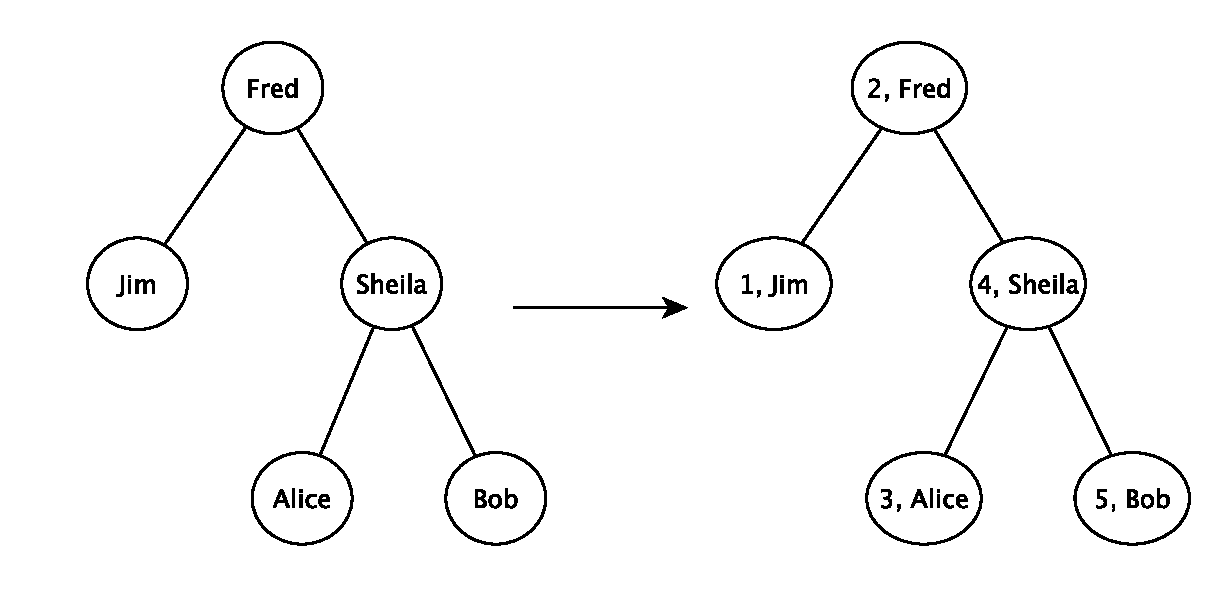
\includegraphics[width=12cm]{content/treelabel.pdf}
\end{center}

\noindent
We can describe binary trees with the following data type \texttt{BTree}
and \texttt{testTree} to represent the example input above:

\begin{code}
data BTree a = Leaf
             | Node (BTree a) a (BTree a)

testTree : BTree String
testTree = Node (Node Leaf "Jim" Leaf)
                "Fred"
                (Node (Node Leaf "Alice" Leaf)
                      "Sheila"
                      (Node Leaf "Bob" Leaf))
\end{code}

\noindent
Then our function to implement tagging, beginning to tag with a specific
value \texttt{i}, has the following type:

\begin{code}
treeTag : (i : Int) -> BTree a -> BTree (Int, a)
\end{code}

\subsubsection*{First attempt}

Na\"{i}vely, we can implement \texttt{treeTag} by implementing a helper
function which propagates a counter, returning the result of the count for
each subtree:

\begin{code}
treeTagAux : (i : Int) -> BTree a -> (Int, BTree (Int, a))
treeTagAux i Leaf = (i, Leaf)
treeTagAux i (Node l x r)
       = let (i', l') = treeTagAux i l in
         let x' = (i', x) in
         let (i'', r') = treeTagAux (i' + 1) r in
             (i'', Node l' x' r')
  
treeTag : (i : Int) -> BTree a -> BTree (Int, a)
treeTag i x = snd (treeTagAux i x)
\end{code}

\noindent
This gives the expected result when run at the \Idris{} REPL prompt:

\begin{code}
*TreeTag> treeTag 1 testTree 
Node (Node Leaf (1, "Jim") Leaf)
     (2, "Fred")
     (Node (Node Leaf (3, "Alice") Leaf)
           (4, "Sheila")
           (Node Leaf (5, "Bob") Leaf)) : BTree (Int, String)
\end{code}

\noindent
This works as required, but there are several problems when we try to scale
this to larger programs. It is error prone, because we need to ensure that
state is propagated correctly to the recursive calls (i.e. passing the
appropriate \texttt{i} or \texttt{i'}). It is hard to read, because the
functional details are obscured by the state propagation. Perhaps most
importantly, there is a common programming pattern here which should be
abstracted but instead has been implemented by hand. There is local mutable
state (the counter) which we have had to make explicit.

\subsection{Introducing \effects{}}

\Idris{} provides a library, \effects{}~\cite{brady-icfp2013}, which captures
this pattern and many others involving effectful computation\footnote{The
earlier paper~\cite{brady-icfp2013} describes the essential implementation
details, although the library presented there is an earlier version which is
less powerful than that presented in this tutorial.}. An effectful program
\texttt{f} has a type of the following form:

\begin{code}
f : (x1 : a1) -> (x2 : a2) -> ... -> { effs } Eff m t
\end{code}

\noindent
That is, the return type gives the effects that \texttt{f} supports
(\texttt{effs}, of type \texttt{List EFFECT}), 
the \emph{computation context} it runs in (\texttt{m}) and the
type the computation returns \texttt{t}. The computation context can be
any function of type \texttt{Type -> Type}, for example \texttt{id}. 
When we come to run an effectful program in \texttt{\{ effs \} Eff m t},
the result will be of type \texttt{m t}.
So, our
\texttt{treeTagAux} helper could be written with the following type:

\begin{code}
treeTagAux : BTree a -> { [STATE Int] } Eff id (BTree (Int, a))
\end{code}

\noindent
That is, \texttt{treeTagAux} has access to an integer state, because the
list of available effects includes \texttt{STATE Int}. \texttt{STATE} is
declared as follows in the module \texttt{Effect.State} (that is, we must
\texttt{import Effect.State} to be able to use it):

\begin{code}
STATE : Type -> EFFECT
\end{code}

\noindent
It is an effect parameterised by a type (by convention, we write
effects in all capitals).
The \texttt{treeTagAux} function runs in the
identity computation context and
returns a new tree tagged with \texttt{Ints}. It is implemented as
follows:

\begin{code}
treeTagAux Leaf = pure Leaf
treeTagAux (Node l x r)
    = do l' <- treeTagAux l
         i <- get
         put (i + 1)
         r' <- treeTagAux r
         pure (Node l' (i, x) r')
\end{code}

\noindent
There are several remarks to be made about this implementation. Essentially,
it hides the state, which can be accessed using \texttt{get} and updated using
\texttt{put}, but it introduces several new features. Specifically, it uses
\texttt{do}-notation, binding variables with \texttt{<-}, and a
\texttt{pure} function. There is much to be said about these features, but
for our purposes, it suffices to know the following:

\begin{itemize}
\item \texttt{do} blocks allow effectful operations to be sequenced.
\item \texttt{x <- e} binds the result of an effectful operation \texttt{e} to
a variable \texttt{x}. For example, in the above code, \texttt{treeTagAux l}
is an effectful operation returning a pair \texttt{(Int, BTree a)}, so
\texttt{l'} has type \texttt{(Int, BTree a)}.
\item \texttt{pure e} turns a pure value \texttt{e} into the result of
an effectful operation. 
\end{itemize}

\noindent
The \texttt{get} and \texttt{put} functions read and write a state \texttt{t}, 
assuming that the \texttt{STATE t} effect is available. They have the following
types, polymorphic in the state \texttt{t} they manage and the context
\texttt{m} in which they run:

\begin{code}
get :      { [STATE t] } Eff m t
put : t -> { [STATE t] } Eff m () 
\end{code}

\noindent
A program in \texttt{Eff} can call any other function in \texttt{Eff} provided
that the calling function supports at least the effects required by the called
function. In this case, it is valid for \texttt{treeTagAux} to call both
\texttt{get} and \texttt{put} because all three functions support the
\texttt{STATE Int} effect.

To run a program in \texttt{Eff} (that is, to evaluate it in an appropriate
context), we use the \texttt{run} or \texttt{runPure} function. Using 
\texttt{runPure}, which runs an effectful program in the identity context,
we can write the \texttt{treeTag} function as follows, using \texttt{put}
to initialise the state:

\begin{code}
treeTag : (i : Int) -> BTree a -> BTree (Int, a)
treeTag i x = runPure (do put i
                          treeTagAux x)
\end{code}

\noindent
We could also run the program in an impure context, such as \texttt{IO},
by changing the type of \texttt{treeTagAux} to be polymorphic in computation
contexts, and using \texttt{run} instead of \texttt{runPure}:

\begin{code}
treeTagAux : BTree a -> { [STATE Int] } Eff m (BTree (Int, a))
...

treeTag : (i : Int) -> BTree a -> IO (BTree (Int, a))
treeTag i x = run (do put i
                      treeTagAux x)
\end{code}

\noindent
Note that the definition of \texttt{treeTagAux} is exactly as before. All that
has changed is that the type is more generic, and can run in \emph{any}
computation context \texttt{m}. There are no constraints on \texttt{m} other
than that it must have type \texttt{Type -> Type}. For reference, this
complete program (including a \texttt{main} to run it) is shown in
Listing \ref{introprog}.


\begin{code}[float=h,frame=single,caption={Tree tagging}, label=introprog]
module Main

import Effect.State

data BTree a = Leaf
             | Node (BTree a) a (BTree a)

instance Show a => Show (BTree a) where
    show Leaf = "[]"
    show (Node l x r) = "[" ++ show l ++ " "
                            ++ show x ++ " "
                            ++ show r ++ "]"

testTree : BTree String
testTree = Node (Node Leaf "Jim" Leaf)
              "Fred"
              (Node (Node Leaf "Alice" Leaf)
                    "Sheila"
                    (Node Leaf "Bob" Leaf))

treeTagAux : BTree a -> { [STATE Int] } Eff m (BTree (Int, a))
treeTagAux Leaf = pure Leaf
treeTagAux (Node l x r)
  = do l' <- treeTagAux l
       i <- get
       put (i + 1)
       r' <- treeTagAux r
       pure (Node l' (i, x) r')

treeTag : (i : Int) -> BTree a -> BTree (Int, a)
treeTag i x = runPure (do put i
                          treeTagAux x)

main : IO () 
main = print (treeTag 1 testTree) 
\end{code}


\subsection{Effects and Resources}

Each effect is associate with a \emph{resource}, which is initialised before
an effectful program can be run. For example, in the case of \texttt{STATE Int}
the corresponding resource is the integer state itself.
The types of \texttt{runPure} and \texttt{run} show this (slightly
simplified here for illustrative purposes):

\begin{code}
runPure : {env : Env id xs} -> { xs } Eff id a -> a
run : Applicative m => {env : Env m xs} -> { xs } Eff m a -> m a
\end{code}

\noindent
The \texttt{env} argument is implicit, and initialised automatically where
possible using default values given by instances of the following type class:

\begin{code}
class Default a where
    default : a
\end{code}

\noindent
Instances of \texttt{Default} are defined for all primitive types, and many
library types such as \texttt{List}, \texttt{Vect}, \texttt{Maybe}, pairs,
etc. However, where no default value exists for a resource type (for example,
you may want a \texttt{STATE} type for which there is no \texttt{Default}
instance) the resource environment can be given explicitly using one of
the following functions:

\begin{code}
runPureInit : Env id xs -> { xs } Eff id a -> a
runInit : Applicative m => Env m xs -> { xs } Eff m a -> m a
\end{code}

\noindent
To be well-typed, the environment must contain resources corresponding exactly
to the effects in \texttt{xs}.
For example, we could also have implemented \texttt{treeTag} by initialising
the state as follows:

\begin{code}
treeTag : (i : Int) -> BTree a -> BTree (Int, a)
treeTag i x = runPureInit [i] (treeTagAux x)
\end{code}

\subsection{Labelled Effects}

What if we have more than one state, especially more than one state of the
same type? How would \texttt{get} and \texttt{put}
know which state they should be referring to? For example, how could we
extend the tree tagging example such that it additionally counts the number
of leaves in the tree?
%
One possibility would be to change the state so that it captured both of
these values, e.g.:

\begin{code}
treeTagAux : BTree a -> { [STATE (Int, Int)] } Eff m (BTree (Int, a))
\end{code}

\noindent
Doing this, however, ties the two states together throughout (as well as
not indicating which integer is which). It would be nice to be able to
call effectful programs which guaranteed only to access one of the states,
for example. In a larger application, this becomes particularly important.

The \effects{} library therefore allows effects in general to be
\emph{labelled} so that they can be referred to explicitly by a particular
name. This allows multiple effects of the same type to be included. We can
count leaves and update the tag separately, by labelling them as follows:

\begin{code}
treeTagAux : BTree a -> { ['Tag ::: STATE Int,
                           'Leaves ::: STATE Int] } Eff m (BTree (Int, a))
\end{code}

\noindent
The \texttt{:::} operator allows an arbitrary label to be given to an effect.
This label can be any type---it is simply used to identify an effect uniquely.
Here, we have used a symbol type. In general \texttt{'name} introduces a
new symbol, the only purpose of which is to disambiguate values\footnote{In
practice, \texttt{'name} simply introduces a new empty type}. 

When an effect is labelled, its operations are also labelled using the
\texttt{:-} operator. In this way, we can say explicitly which state we mean
when using \texttt{get} and \texttt{put}. The tree tagging program which also
counts leaves can be written as follows:

\begin{code}
treeTagAux Leaf = do 'Leaves :- update (+1)
                     pure Leaf
treeTagAux (Node l x r)
  = do l' <- treeTagAux l
       i <- 'Tag :- get
       'Tag :- put (i + 1)
       r' <- treeTagAux r
       pure (Node l' (i, x) r')
\end{code}

\noindent
The \texttt{update} function here is a combination of \texttt{get} and \texttt{put},
applying a function to the current state.

\begin{code}
update : (x -> x) -> { [STATE x] } Eff m () 
\end{code}

\noindent
Finally, our top level \texttt{treeTag} function now returns a pair of
the number of leaves, and the new tree. Resources for labelled effects are
intialised using the \texttt{:=} operator (reminisicent of assignment in
an imperative language):

\begin{code}
treeTag : (i : Int) -> BTree a -> (Int, BTree (Int, a))
treeTag i x = runPureInit ['Tag := i, 'Leaves := 0]
                    (do x' <- treeTagAux x
                        leaves <- 'Leaves :- get
                        pure (leaves, x'))
\end{code}

\noindent
To summarise, we have:

\begin{itemize}
\item \texttt{:::} to convert an effect to a labelled effect.
\item \texttt{:-} to convert an effectful operation to a labelled effectful operation.
\item \texttt{:=} to initialise a resource for a labelled effect.
\end{itemize}

\noindent
Or, more formally with their types (slightly simplified to account only for
the situation where available effects are not updated):

\begin{code}
(:::) : lbl -> EFFECT -> EFFECT
(:-)  : (l : lbl) -> { [x] } Eff m a -> { [l ::: x] } Eff m a
(:=)  : (l : lbl) -> res -> LRes l res
\end{code}

\noindent
Here, \texttt{LRes} is simply the resource type associated with a labelled
effect. Note that labels are polymorphic in the label type \texttt{lbl}. 
Hence, a label can be anything---a string, an integer, a type, etc.

\subsection{\texttt{!}-notation}

In many cases, using \texttt{do}-notation can make programs unnecessarily
verbose, particularly in cases where the value
bound is used once, immediately. The following program returns the length of
the \texttt{String} stored in the state, for example:

\begin{code}
stateLength : { [STATE String] } Eff m Nat
stateLength = do x <- get
                 pure (length x)
\end{code}

\noindent
This seems unnecessarily verbose, and it would be nice to program in a more
direct style in these cases. \Idris{} provides \texttt{!}-notation to help
with this. The above program can be written instead as:

\begin{code}
stateLength : { [STATE String] } Eff m Nat
stateLength = pure (length !get)
\end{code}

\noindent
The notation \texttt{!expr} means that the expression \texttt{expr} should
be evaluated and then implicitly bound. Conceptually,
we can think of \texttt{!} as being a prefix function with the following type:

\begin{code}
(!) : { xs } Eff m a -> a
\end{code}

\noindent
Note, however, that it is not really a function, merely syntax! In practice, a
subexpression \texttt{!expr} will lift \texttt{expr} as high as possible within
its current scope, bind it to a fresh name \texttt{x}, and replace
\texttt{!expr} with \texttt{x}. Expressions are lifted depth first, left to
right. In practice, \texttt{!}-notation allows us to program in a more direct
style, while still giving a notational clue as to which expressions are
effectful.

For example, the expression\ldots

\begin{code}
let y = 42 in f !(g !(print y) !x) 
\end{code}

\ldots is lifted to:

\begin{code}
let y = 42 in do y' <- print y
                 x' <- x
                 g' <- f y' x'
                 f g'
\end{code}


\subsection{Syntactic Sugar and \texttt{Eff}}

By now, you may be wondering about the syntax we are using for \texttt{Eff},
because it doesn't look like a normal \Idris{} type! (If not, you may
safely skip this section and return to it later.) In fact, the type of
\texttt{Eff} is the following:

\begin{code}
Eff : (m : Type -> Type) ->
      (x : Type) ->
      List EFFECT -> (x -> List EFFECT) -> Type
\end{code}

\noindent
This is more general than the types we have been writing so far. It is
parameterised over a computation context \texttt{m}, a result type \texttt{x},
as we have already seen, but also a \texttt{List EFFECT} and a function type
\texttt{x -> List EFFECT}.

These additional parameters are the list of \emph{input} effects, and a list
of \emph{output} effects, computed from the result of an effectful operation.
That is: running an effectful program can change the set of effects available!
This is a particularly powerful idea, and we will see its consequences in more
detail later. Some examples of operations which can change the set of available
effects are:

\begin{itemize}
\item Updating a state containing a dependent type (for example adding an
element to a vector).
\item Opening a file for reading is an effect, but whether the file really
\emph{is} open afterwards depends on whether the file was successfully opened.
\item Closing a file means that reading from the file should no longer be
possible.
\end{itemize}

\noindent
While powerful, this can make uses of the \texttt{Eff} type hard to read.
Therefore, the \effects{} library provides syntactic sugar which is translated
such that\ldots

\begin{code}
{ xs } Eff m a 
\end{code}

\ldots is expanded to \ldots

\begin{code}
Eff m a xs (\_ => xs)
\end{code}

\noindent
i.e. the set of effects remains the same on output. This suffices for the
\texttt{STATE} example we have seen so far, and for many useful side-effecting
programs. We could also have written \texttt{treeTagAux} with the expanded
type:

\begin{code}
treeTagAux : BTree a -> 
             Eff m (BTree (Int, a)) [STATE Int] (\x => [STATE Int])
\end{code}

\noindent
Later, we will see programs which update effects:

\begin{code}
{ xs ==> xs' } Eff m a
\end{code}

\ldots which is expanded to \ldots

\begin{code}
Eff m a xs (\_ => xs')
\end{code}

\noindent
i.e. the set of effects is updated to \texttt{xs'} (think of a transition
in a state machine). There is, for example, a version of \texttt{put} which
updates the type of the state:

\begin{code}
putM : y -> { [STATE x] ==> [STATE y] } Eff m () 
\end{code}

\noindent
Also, we have:

\begin{code}
{ {res} xs ==> xs' } Eff m a
\end{code}

\ldots which is expanded to \ldots

\begin{code}
Eff m a xs (\res => xs')
\end{code}

\noindent
i.e. the set of effects is updated according to the result of the operation
\texttt{res}.




